\documentclass[11pt]{article}

\usepackage{amsmath, amsfonts, amsthm}
\usepackage{bm}
\usepackage{graphicx}

\newtheorem{theorem}{Theorem}%[section]
\newtheorem{corollary}{Corollary}%[theorem]
\newtheorem{lemma}[theorem]{Lemma}
\newtheorem{proposition}{Proposition}


\begin{document}
\title{$\ell^0$-norm, $\ell^1$-norm and $\ell^4$-norm in $S^1$}
\author{Kwan Ho Ryan Chan\\Department of Electrical Engineer \& Computer Science\\University of California, Berkeley}
\maketitle

\section{Source Code}
	The code used to generate the following plots are uploaded to Github. Link: \texttt{https://github.com/ryanchankh/L0L1L4NormS1}
\section{Introduction}
Suppose we have an optimization problem as follows:
\begin{equation}
\begin{aligned}
     & \underset{||\bm{x}||_2=1}{\text{argmin}} & ||\bm{x}||_0  \label{eq:1}
\end{aligned}
\end{equation}
In plain words, we are trying to find the sparsest solution (most 0's entries), such that the solution
is a point on the sphere $S^1$. This problem is NP-hard. So a natural way to solve this is by relaxing the problem to another form. The goal of this article is to show how the solutions to (\ref{eq:1}) corresponds to solving the following: \\
Case 1:
\begin{equation}
\begin{aligned}
     & \underset{||\bm{x}||_2=1}{\text{argmin}} & ||\bm{x}||_1^2  \label{eq:2}
\end{aligned}
\end{equation}
Case 2:  
\begin{equation}
\begin{aligned}
     & \underset{||\bm{x}||_2=1}{\text{argmax}} & ||\bm{x}||_4^4  \label{eq:3}
\end{aligned}
\end{equation}
Note that raising them to even powers does not change the solution. Notice for $\ell^1$-norm, the problem is a minimization. But for $\ell^4$-norm, it is a maximization. Miraculously, their solutions converge, and both corresponds to the best approximation to (\ref{eq:1}).  

\section{Prerequisites}
For clarification, we say $\bm{x}$ is sparser than $\bm{y}$ if there are more 0 entries in $\bm{x}$ than in $\bm{y}$. 

To make the proof make sense, let us first show a simple lemma:
\begin{lemma}\label{eq:4}
    For any $\bm{x} = (x_1, x_2, \cdots, x_n)$, the following expression is true. 
    \begin{equation}
        (\sum^n_{i=1} x_i)^2 = \sum^n_{i=1} x_i^2 + 2\sum^n_{i < j} x_ix_j
    \end{equation}
\end{lemma}
\begin{proof}
    It is easy to see once we express the summation in an specific tabular way:
    \begin{align*}
        (\sum^n_{i=1} x_i)^2 
        &= (\sum^n_{i=1} x_i)(\sum^n_{i=1} x_i) \\
        &= \sum^n_{i=1} \sum^n_{j=1} x_i x_j \\
        &= x_1x_1 + x_1x_2 + \cdots + x_1x_n \\
        & + x_2x_1 + x_2x_2 + \cdots + x_2x_n \\ 
        & + \cdots \\
        & + x_nx_1 + x_2x_2 + \cdots + x_nx_n \\
        & = \sum^n_{i=1} x_i^2 + 2\sum^n_{i < j} x_ix_j
    \end{align*}
    by breaking the expression into the sum of diagonals and off-diagonals.
\end{proof}

Moreover, we can actually raise all $x_{i}$ to a certain power, and generalize the expression to the following:
\begin{equation}
	(\sum^n_{i=1} x_i^{k})^2 = \sum^n_{i=1} ((x_i)^{k})^2 + 2\sum^n_{i < j} (x_i)^{k}(x_j)^{k}
\end{equation}

Another lemma we need to know, is the following about square roots:
\begin{lemma} For any $\bm{x} = (x_1, x_2, \cdots, x_n)$, the following inequality is true:
    \begin{equation}\label{eq:5}
        \sum^n_{i=1} \sqrt{(x_i)^2} \geq \sqrt{\sum^n_{i=1} (x_i)^2} 
    \end{equation}
\end{lemma}

The proof is fairly simple, so we will leave this to the reader.


\section{Case 1: $\ell^1$-norm Minimization}

\subsection{Algebraic Explanation}
To find the bound for $||\bm{x}||_1$, we expand the terms for $||\bm{x}||_1^2$, then we get:
\begin{align*}
    ||\bm{x}||_1^2 
        &= \sum^n_1 |x_i| \\
        &= \sum^n_1 \sqrt{(x_i)^2} \\
        &\geq \sqrt{\sum^n_1 (x_i)^2} & \text{(by (\ref{eq:5}))}\\
        &= ||x||_2 \\
        &= 1 & \text{(by $S^1$ constraint)}
\end{align*}
Hence, we have shown that 1 is the lower bound for $||\bm{x}||_1$.

If we expand the expression using (\ref{eq:4}), we get:
\begin{align*}
    ||\bm{x}||_1^2
        &= (\sum^n_{i=1}|x_i|)^2 \\
        &= \sum^n_{i=1} |x_i|^2 + 2 \sum^n_{i=1}|x_i||x_j|
\end{align*}
One can see that if we set $\bm{x}$ as any vector that is not a canonical vector, then $||\bm{x}||_1^2$ will be larger than 1. 

\subsection{Geometric Explanation}
    \begin{figure}[h]
        \centering
        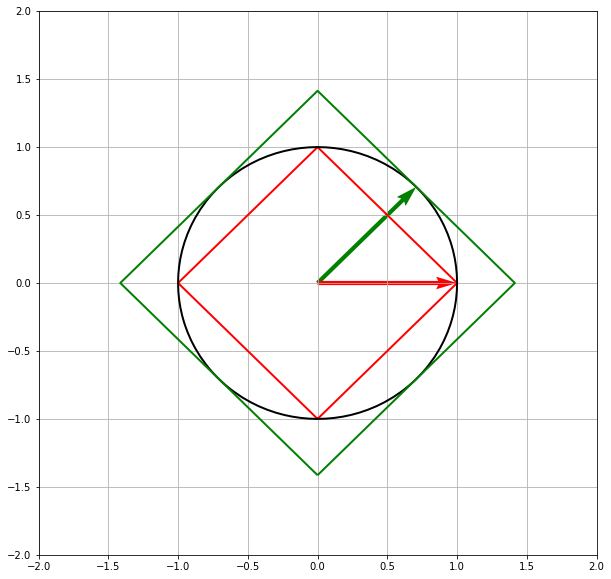
\includegraphics[scale=0.4]{l1norm_bound.png}
        \caption{$\ell^{1}$-norm minimization visualization}
        \label{fig:l1_bound}
    \end{figure}
    One can visualize the relationship of $\ell^1$-norms by considering different vectors on $S^1$. For example, let's turn to figure \ref{fig:l1_bound}. Assume we are living in $\mathbb{R}^2$. The geometry of $\ell^1$-norm is a diamond. The red arrow is the vector $(1, 0)$, which is one of the solution to our optimization problem. And the green arrow is the vector $(\sqrt{2}, \sqrt{2})$. We can see that both red and green arrow lives in $S^1$, but when we graph out the relative $\ell^1$-norm diamond, we can see that the green diamond is bigger than the red diamond. Moreover, this generalizes to any vector that lives in $S^1$. 


\section{Case 2: $\ell^4$-norm Maximization}
	As we will see later, the proofs are nearly identical as the $\ell^{1}$ case.

\subsection{Algebraic Explanation}
	To find the bound for $||\bm{x}||_1$, we expand the terms for $||\bm{x}||_1^2$, then we get:
	\begin{align}
    	||\bm{x}||_4^4 
    		&= \sum^{n}_{i=1} |x_{i}|^{4} \\
			&\leq \sum^{n}_{i=1} ((x_{i})^{2})^{2} + 2\sum^{n}_{i<j} x_{i}^{2}x_{j}^{2}\label{eq:7}\\
			&= (\sum^{n}_{i=1} (x_{i})^2)^{2} \\
			&= 1
	\end{align}
	Although this seem less intuitive, we can observe the properties of the expressions we derived. Here, the $||\bm{x}_{4}||^{4}$
	is now upper bounded by 1. Moreover, we show equation (\ref{eq:7}) = 1, and $2\sum^{n}_{i<j} x_{i}^{2}x_{j}^{2}$
	is minimum if and only if $\sum^{n}_{i=1} ((x_{i})^{2})^{2}$ is maximum. Since $2\sum^{n}_{i<j} x_{i}^{2}x_{j}^{2}$ is at minimum 
	if it has 0's, this implies that $||\bm{x}||_4^4$ is maximum when $\bm{x}$ is a canonical vector. 
	

\subsection{Geometric Explanation}
    \begin{figure}[h]
        \centering
        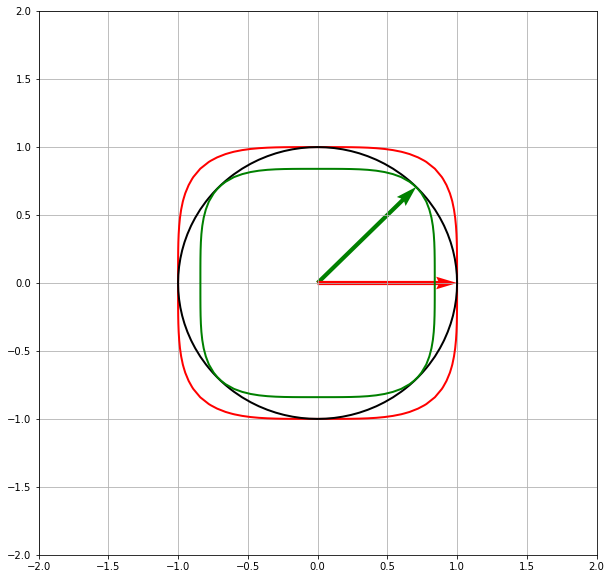
\includegraphics[scale=0.4]{l4norm_bound.png}
        \caption{$\ell^{4}$-norm maximization visualization}
        \label{fig:l4_bound}
    \end{figure}
    Similar to our previous visualization for the $\ell^{1}$-norm, the red vector here is the canonical vector, and the green 
    vector is the diagonal. The shape of $\ell^{4}$-ball is a rounded square. One can see that if we choose a vector that is not 
    a canonical vector, like the green vector, the green rounded square is always smaller than the red rounded square. 
    
\section{Conclusion}
	What we presented here might seem like very simple concepts. $\ell^{p}$-norm is an operation used all over optimization, 
	linear algebra, metric differential geometry, etc. It is important to be to see the same topic from all kinds of perspective. 
	I hope this short write-up reveals something interesting to you, as this is also a reminder to me just in case if I forget about 
	this in the future lol. 





\end{document}
